\documentclass[main]{subfiles}
\begin{document}

%@@@@@@@@@@@@@@@@@@@@@@@@@@@@@@
% Main Topics: Plasticity and Learning 08.11.2018
% Lecturer: Daniel Kiper
% author: Vanessa Leite - base document from benelot/eth-intro-to-neuroinformatics-summary

\section{Modeling Synapses}

\begin{figure}[H]
	\centering
 	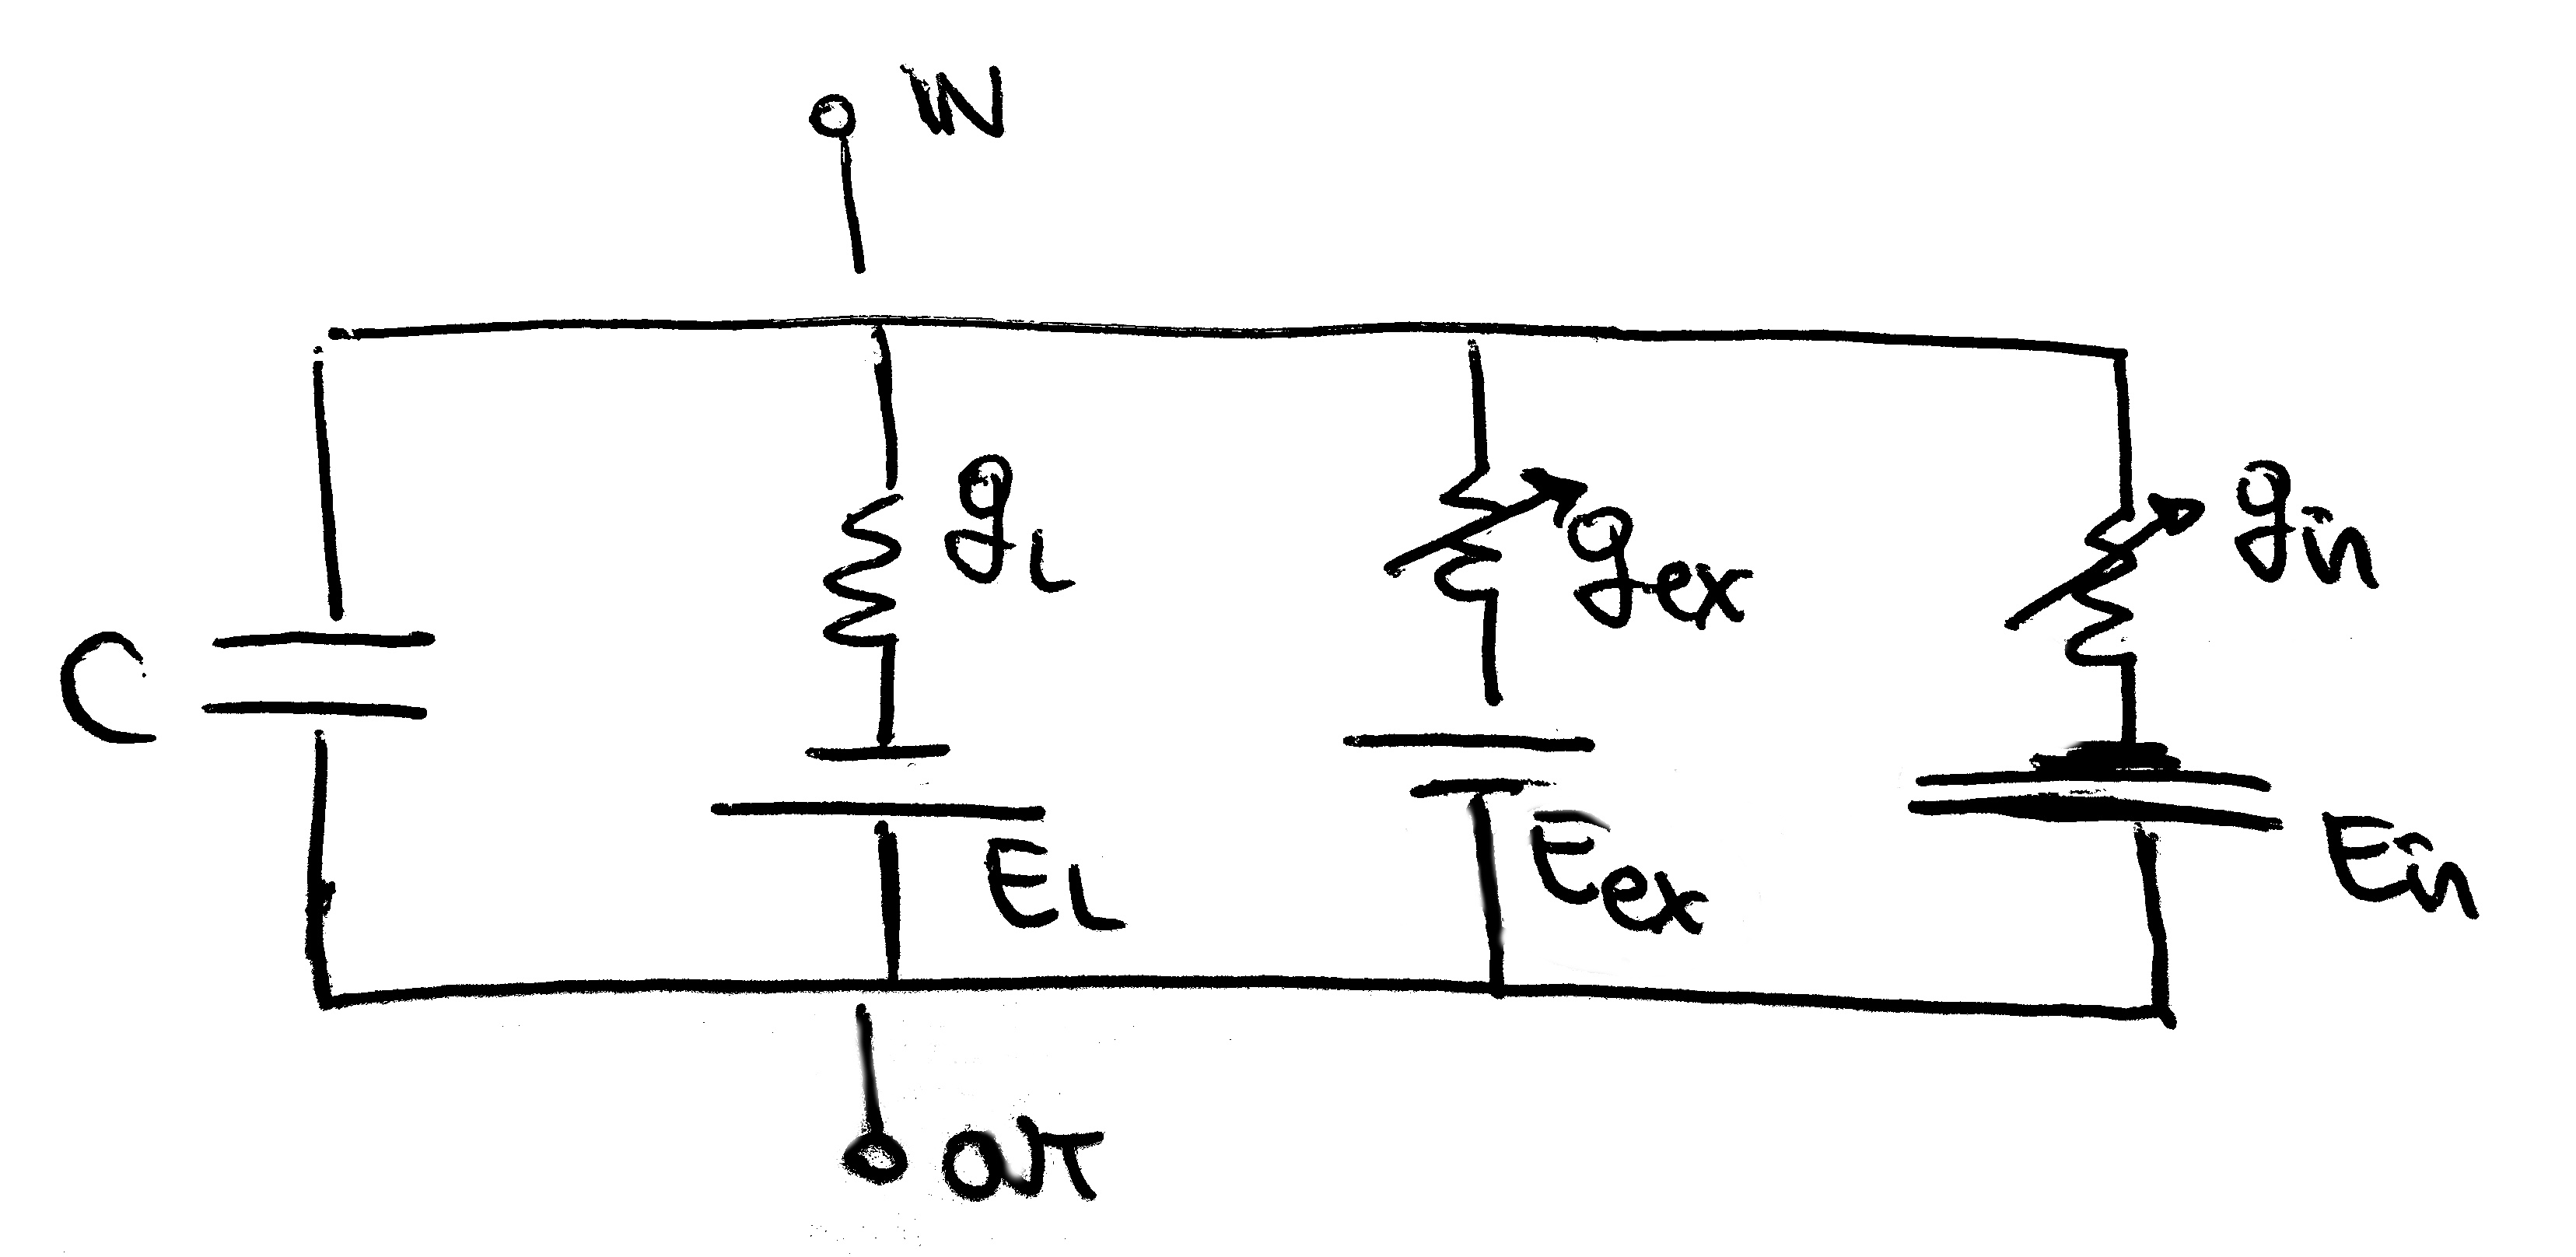
\includegraphics[width=0.5\textwidth]{synapse-model.jpg}
 	\caption{Synapse model}
 	\label{fig:synapse-model}
\end{figure}

\subsubsection{$E_{syn}$ and $E_{th}$}
\begin{itemize}
\item $E_{syn} > E_{th}$: excitatory
\item $E_{syn} < E_{L}$: inhibitory
\item $E_{syn} \approx E_{L}$: shuting inhibition
\end{itemize}

Voltage Clamp experiments (excitatory synapse): synapse input is well captured by Ohm Law's.

Modified membrane patch equation with a synapse:
\[ C \frac{dV_m}{dt} + g_{syn}(t)(V_m - E_{syn}) + \frac{V_m - V_{rest}}{R} = 0 \]
Rewriting:
\[ \tau \frac{dV_m}{dt} = -(1 + R g_{syn}(t)) V_m + R g_{syn}(t) E_{syn} + V_{rest} \]
where $\tau = RC$.

\subsection{Alpha function}
Synapse input is usually approximated by an ``alpha function": $g_{syn} = g_{peak} t exp(\frac{-t}{t_{peak}}$.

\begin{figure}[H]
	\centering
 	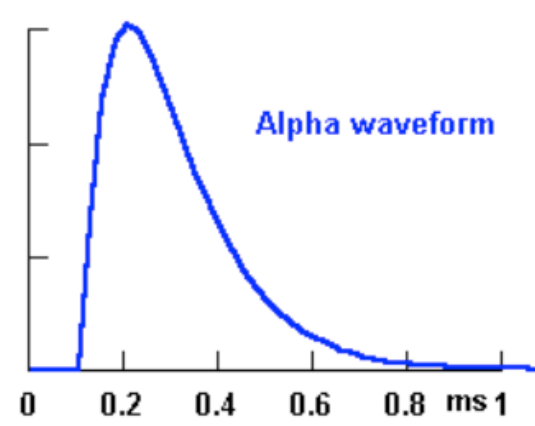
\includegraphics[width=0.3\textwidth]{alpha-waveform.png}
\end{figure} 

To model many synaptic input, we add them in parallel to a RC circuit. This way:
\[ C \frac{dV_m}{dt} = \sum_{i=0}^{n} g_{syn, i}(t) (E_{syn, i} - V_m) + \frac{V_{rest} -V_m}{R} \]

Considering the synaptic input varying slowly: $g_{syn}(t) \approx g_{syn}$. Also, if $V_m << E_{syn}$, the synaptic input can be approximated as a const current source: $g_{syn} \cdot E_{syn})$. Then:

\[ \tau\prime \frac{dV_m}{dt} = -V + \frac{g_{syn}E_{syn}}{G_{in}} \]
where, $\tau\prime = \frac{C}{G_{in}}$ and $G_{in} = g_{syn} + \frac{1}{R}$.

That leads to:
\[ V_\infty = \frac{R g_{syn} E_{syn}}{1 + R g_{syn}} \]

\subsubsection{Small synaptic input}
Voltage scales linearly with synaptic input.
$Rg_{syn} << 1 \rightarrow V_\infty = R g_{syn} E_{syn}$

\subsubsection{Large synaptic input}
Voltage saturates at synaptic reversal potential.
$Rg_{syn} >> 1 \rightarrow V_\infty = E_{syn}$

\subsection{Shunting inhibition}
Special case when the synapse reversal potential is equal to the resting membrane potential.

Consider the scheme in Figure~\ref{fig:synapse-model}. We have an excitatory and an inhibitory synapse.

\[ C \frac{dV}{dt} = g_{ex}(E_{ex} - V) - g_{in} V - \frac{V}{R} \]

Rewriting,

\[ \tau\prime \frac{dV}{dt} = -V + \frac{g_{ex}E_{syn}}{G_{in}} \]
where, $\tau\prime = \frac{C}{G_{in}}$ and $G_{in} = g_{ex} + g_{in} + \frac{1}{R}$.

\[ V(t) = \frac{g_{ex} E_{ex}}{G_{in}} (1 - e^{\frac{-t}{\tau\prime}} \]

\[ V_\infty = \frac{g_{ex} E_{ex}}{g_{ex} + \frac{1}{R} + g_{in}} \]

Notice, $g_{in}$ only appears in the denominator. 
Shunting inhibition is also called ``divisive inhibition".
The strong the inhibition, smaller is the voltage.

\subsection{Plasticity (Hebb's Law) - 1940's}
Neurons that fire together, wire together.

\subsubsection{Spike-time dependent plasticity}
\begin{figure}[H]
	\centering
 	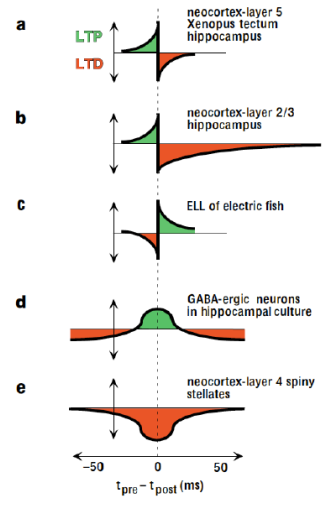
\includegraphics[width=0.5\textwidth]{spike-time-dependent-plasticity.png}
\end{figure}


\end{document}
